\documentclass{article}
\usepackage{geometry}
\usepackage{graphicx}
\usepackage[pages=some]{background}
\usepackage{titling}
\usepackage{tabularx}
\usepackage{tikz}
\usepackage{forest}

\forestset{
  my box/.style={
    draw,
    rectangle,
    rounded corners,
    fill=gray!20,
    inner sep=6pt,
    minimum width=3cm % Adjust the width as needed
  }
}


\geometry{a4paper}

\backgroundsetup{
    scale=1,
    angle=0,
    opacity=1,
    contents={%
        \includegraphics[width=\paperwidth,height=\paperheight]{institution_logo.jpg}
    }
}

\newcommand{\subtitle}[1]{
    \posttitle{
        \par\end{center}
        \begin{center}\large#1\end{center}
        \vskip0.5em}
}

\title{ME-463}
\author{Md. Hasibul Islam}
\subtitle{PETROLEUM ENGINEERING}

\begin{document}
\begin{titlepage}
    \centering
    
    {\Huge\bfseries\maketitle}
    \textbf{Quamrul Islam Sir} \\
    \vspace{2cm}
    \includegraphics[width=8cm]{institution_logo.jpg}
    \vfill
    \vspace*{2cm}
\end{titlepage}

\tableofcontents
\pagebreak
\section{Lecture 01: Introduction} 
\subsection*{\hfill Date: 03/06/2023}

\subsection*{Booklist}

\textbf{Introduction of Petroleum Geology \& Drilling}

\hfill Published by BUET

\subsection*{Basics}

\begin{tabular}{@{}p{1\textwidth}@{}}
Latin: \textbf{Petra} → Rock or Stone \\
Latin: \textbf{Oleum} → Oil \\
So, Petroleum basically means "Rock Oil"\\
\\

Petroleum occurs widely in the earth as gas, liquid, semi-solid or solid, or in more than one state in a single place.
\end{tabular}
\\

\subsection*{Definition}
Chemically, any petroleum is an extremely complex mixture of hydrocarbon (hydrogen and carbon) compounds with minor amounts of nitrogen, oxygen, and sulfur as impurities. The weight percentage of petroleum is as follows:
\\
\begin{center}
\begin{tabularx}{\textwidth}{X X}
  \hline
  \textbf{Elements} & \textbf{Amount} \\
  \hline
  Carbon & 85\%-90\% \\
  Hydrogen & 10\%-15\% \\
  Sulfur & 0.2\%-5\% \\
  $N_{2}$ & 0.1\%-2\% \\
  $O_{2}$ & 0.6\%-2\% \\
  \hline
\end{tabularx}
\end{center}

\vspace{1cm}
% trees 
\begin{center}
  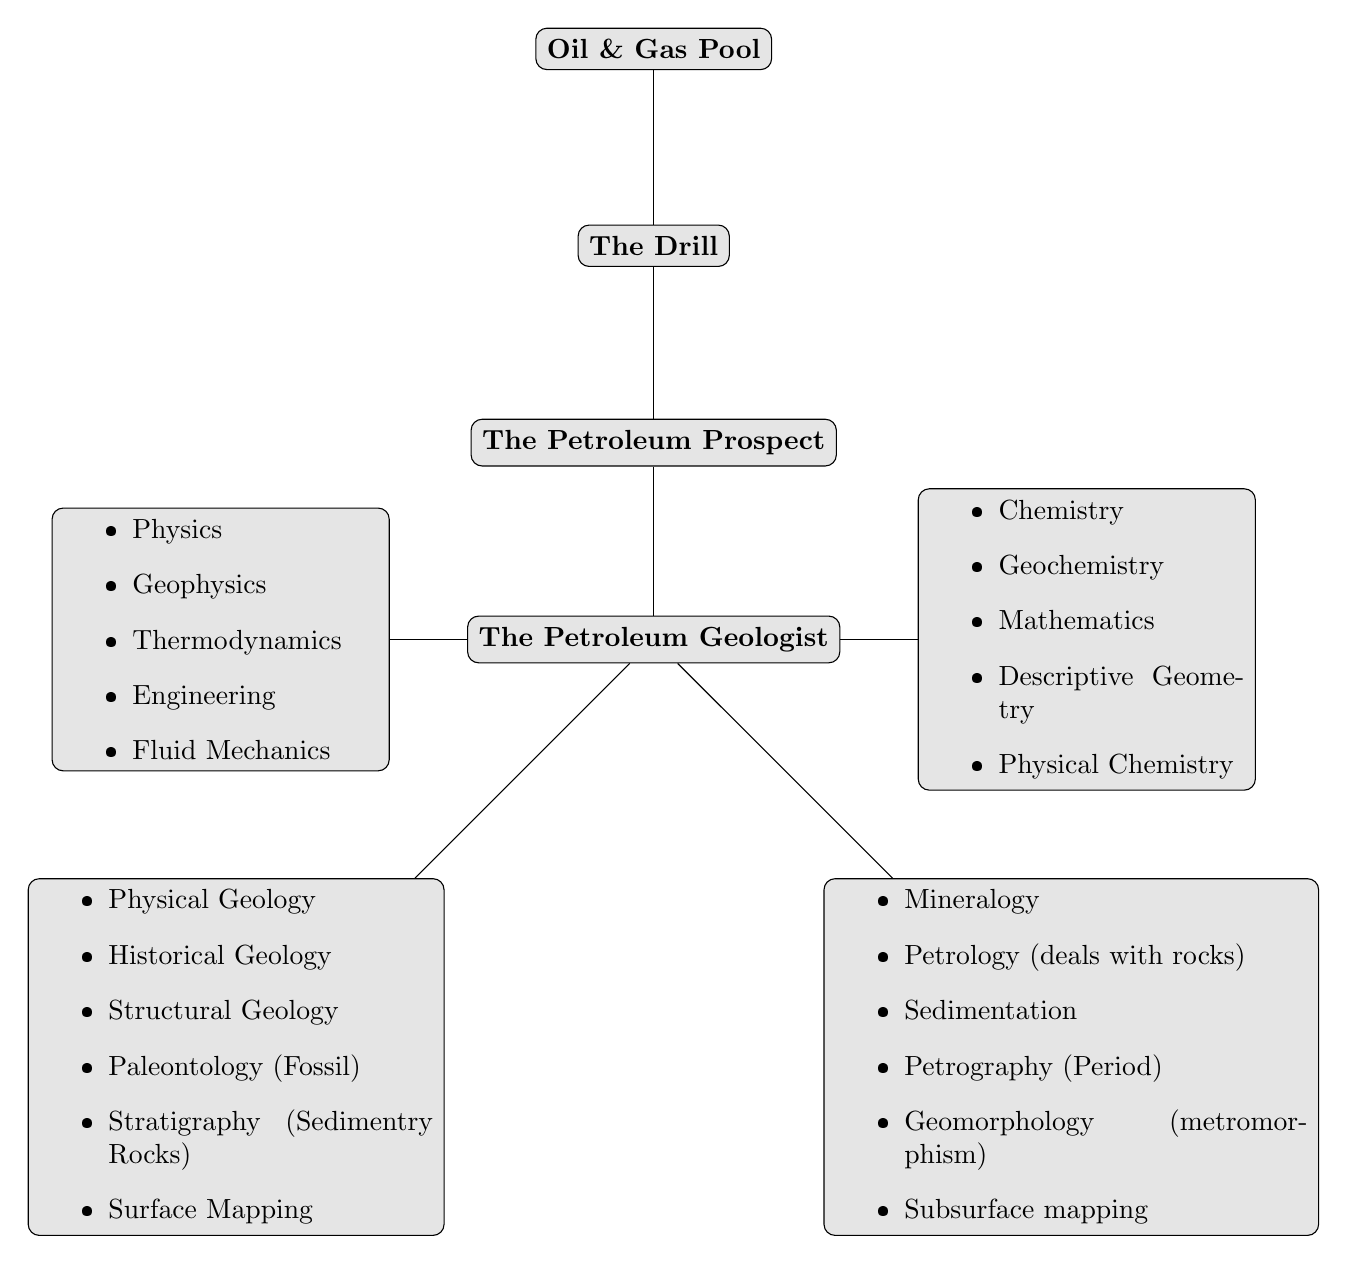
\begin{tikzpicture}[level distance=2cm,
    level 1/.style={sibling distance=2cm},
    level 2/.style={sibling distance=2cm},
    level 4/.style={sibling distance=4cm}, % Adjust the sibling distance for level 4
    box/.style={draw, rectangle, rounded corners, fill=gray!20, inner sep=4pt}]
    \node[box] {\textbf{Oil \& Gas Pool}}
      child[grow=down, level distance=2.5cm] {node[box] {\textbf{The Drill}} % Changed level one node label
        child[grow=down, level distance=2.5cm] {node[box] {\textbf{The Petroleum Prospect}}
          child[grow=down, level distance=2.5cm] {node[box] {\textbf{The Petroleum Geologist}}
            child[grow=left, level distance=5.5cm] {node[box] {
              \begin{minipage}{4cm}
                \begin{itemize}
                  \item Physics
                  \item Geophysics
                  \item Thermodynamics
                  \item Engineering
                  \item Fluid Mechanics
                \end{itemize}
              \end{minipage}
            }}
            child[grow=south west, level distance=7.5cm] {node[box] {
              \begin{minipage}{5cm}
                \begin{itemize}
                  \item Physical Geology
                  \item Historical Geology
                  \item Structural Geology
                  \item Paleontology (Fossil)
                  \item Stratigraphy (Sedimentry Rocks)
                  \item Surface Mapping
                \end{itemize}
              \end{minipage}            
            }}
            child[grow=south east, level distance=7.5cm] {node[box] {
              \begin{minipage}{6cm}
                \begin{itemize}
                  \item Mineralogy
                  \item Petrology (deals with rocks)
                  \item Sedimentation
                  \item Petrography (Period)
                  \item Geomorphology (metromorphism)
                  \item Subsurface mapping
                \end{itemize}
              \end{minipage}            
            }}
            child[grow=right, level distance=5.5cm] {node[box] {
              \begin{minipage}{4cm}
                \begin{itemize}
                  \item Chemistry
                  \item Geochemistry
                  \item Mathematics
                  \item Descriptive Geometry
                  \item Physical Chemistry
                \end{itemize}
              \end{minipage}            
            }}
          }
        }
      };
  \end{tikzpicture}
\end{center}

\vspace{2cm}
\subsection*{Petroleum Geology}
Geology is the sciecne that deals with the history and structure of the earth and its life forms. It is used to credit where oil accumulation might occur. Geology is based on observation and the knowledge derived from mant others sources.
\\

% horizontal tree

\begin{center}
  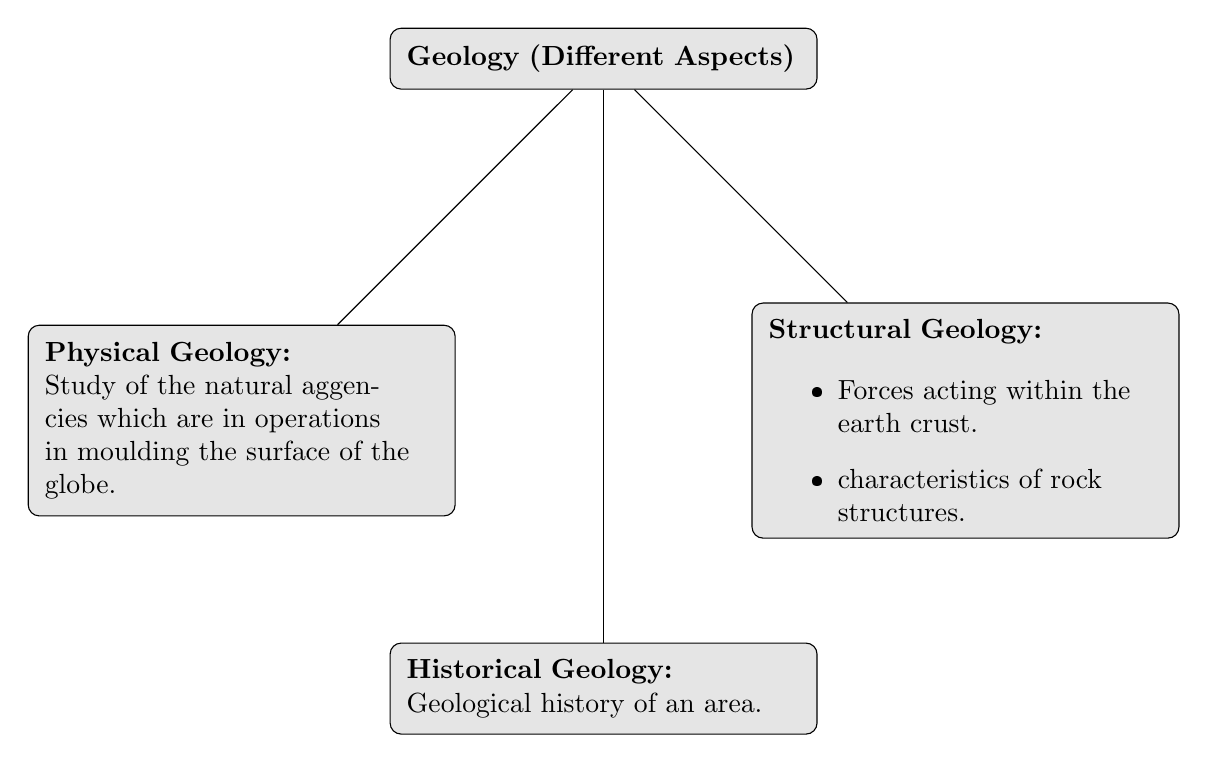
\begin{tikzpicture}[level distance=5cm,
    level 1/.style={sibling distance=5cm},
    level 2/.style={sibling distance=5cm},
    level 3/.style={sibling distance=5cm},
    box/.style={draw, rectangle, rounded corners, fill=gray!20, inner sep=6pt, text width=5cm}]
    \node[box] {\textbf{Geology (Different Aspects)}}
           child[grow=south west, level distance=6.5cm] {node[box] {
        \textbf{Physical  Geology:}\\ 
        Study of the natural aggencies which are in operations in moulding the surface of the globe.
      }}
      child[grow=down, level distance=8cm] {node[box] {
        \textbf{Historical Geology:} \\
        Geological history of an area.
      }}
      child[grow=south east, level distance=6.5cm] {node[box] {
        \textbf{Structural Geology:} \\
        \begin{itemize}
                  \item Forces acting within the earth crust.
                  \item characteristics of rock structures.
                  \end{itemize}
}};
  \end{tikzpicture}
\end{center}
\vspace{2cm}
\subsection*{Petroleum Geologiest (activities)}
\begin{center}
\begin{itemize}
    \item Observes the rock and rock formations.
     \item Reconstructs the geological history of an area 
     \item Determines whether the formations contains petroleum in the reservoirs. 
\end{itemize}
\end{center}



\newpage

\section{Lecture 2: Topic}
\subsection*{Date: DD/MM/YYYY}

Content of the lecture goes here.

\end{document}
